\chapter{Optik}
\[ \underbrace{\SI{750}{\nano\metre}}_{\color{red} rot} < \lambda < \underbrace{\SI{400}{\nano\metre}}_{\color{blue} blau} \]
Ausbreitungsgeschwindigkeit
\[
	c = \frac{c_0}{n} \\
	n = \text{ Brechungsindex} \\
	n \geq 1 \\
	n_{\text{Luft}} = 1 + 3 \cdot 10^{-4} \\
	n_{\ce{H2O}} = 1.33 \\
	n_{\text{Biomat.}} = 2.42 \\
	n_{\text{Vakuum}} \equiv 1
\]

\section{Wellenausbreitung in 2D und 3D}
2 F�lle:
\begin{description}
	\item[Kugelwellen] 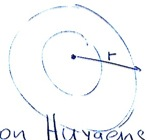
\includegraphics{Bild244}
	\item[ebene Wellen] 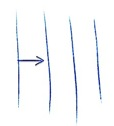
\includegraphics{Bild245}
\end{description}

\subsection{Prinzip von Huygens}
\begin{satz*}
	Jeder Punkt des Mediums das von der Welle erreicht wird, erzeugt eine Kugelwelle derselben Frequenz.
\end{satz*}

\section{Reflexion \& Brechung}
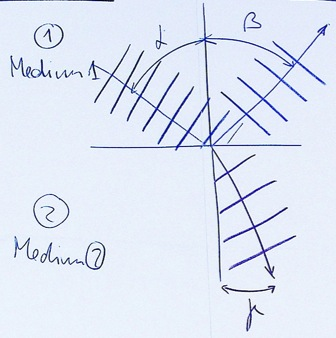
\includegraphics{Bild246}
\[
	\boxed{ \alpha = \beta }\\
	\boxed{ \frac{\sin \alpha}{\sin \beta} = \frac{c_1}{c_2} = \frac{n_2}{n_1} }
\]

\subsection{\enquote{Snellius}}
Totalreflexion
\[ \boxed{ \sin \gamma \geq \frac{n_2}{n_1} } \]

\section{optische Abbildungen}
\subsection{reeler Bildpunkt}
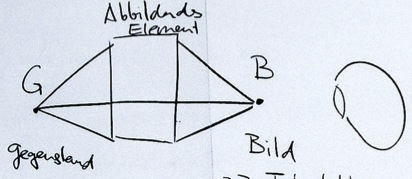
\includegraphics{Bild247} \\
\begin{bsp*}[ head = z.B. ]
	\begin{itemize}
		\item Fotoplatte
		\item CCD Chip
	\end{itemize}
\end{bsp*}

\subsection{virtueller Bildpunkt}
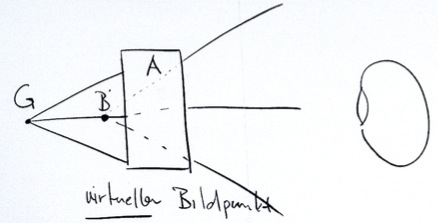
\includegraphics{Bild248} \\
\begin{bsp*}[ head = z.B. ]
	Spiegelbild
\end{bsp*}

\subsection{Abbildungen durch Linsen}
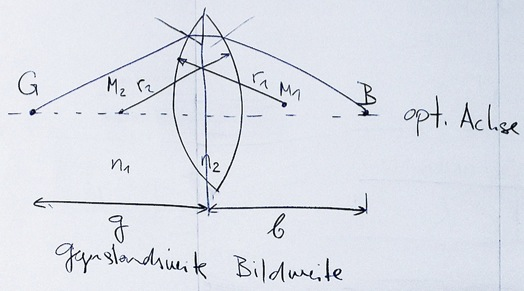
\includegraphics{Bild249} \\
Brennpunkt (e) \\
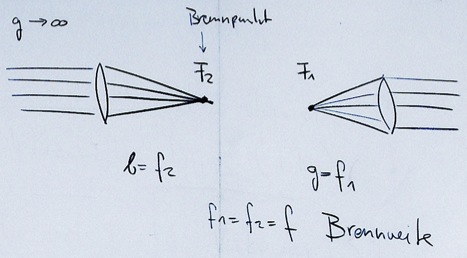
\includegraphics{Bild250} \\
$f_1 = f_2 = f$ Brennweite

\subsubsection{Brechkraft}
\[ D = \frac{1}{f} \overset{=}{\text{d�nne Linse}} \frac{n_2 - n_1}{n_1} \left( \frac{1}{r_1} - \frac{1}{r_2} \right) \]
\begin{bsp*}
	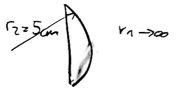
\includegraphics{Bild251} \\
	\begin{itemize}[ label = $\implies$ ]
		\item 10 \uline{Dioptrien} $[ \si[ per-mode = reciprocal ]{\per\metre} ]$
		\item $f = \SI{10}{\centi\metre}$
	\end{itemize}
\end{bsp*}

\subsubsection{Bildkonstuktion}
(via Brennpunkt)
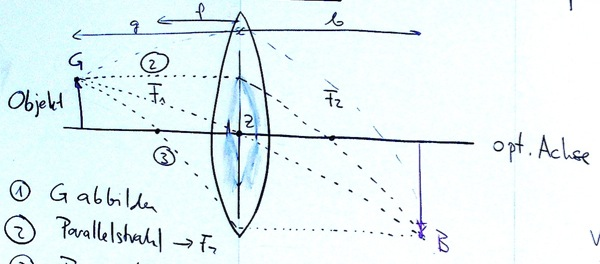
\includegraphics{Bild252} \\
\begin{enumerate}
	\item $G$ abbilden
	\item Parallelstrahl $\rightarrow F_1$
	\item Brennstrahl $\rightarrow F_2$
	\item Kontrollstrahl durch Zentrum
\end{enumerate}

\subsubsection{Abbildungsgleichung}
\[ \boxed{ \frac{1}{g} + \frac{1}{b} = \frac{1}{f} } \]

\subsubsection{Vergr�sserung}
\[
	\boxed{ m = \frac{B}{G} = -\frac{b}{g} } \\
	g > 0 \text{ f�r $G$ links} \\
	b > 0 \text{ f�r $B$ rechts}
\]

\begin{rep*}[ note = Abbildungen mit Linsen ]
	\uline{Brechkraft}
	\[ \boxed{ \phi = \frac{1}{f} = \frac{n_2 - n_1}{n_1} \left( \frac{1}{r_1} - \frac{1}{r_2} \right) } \]
	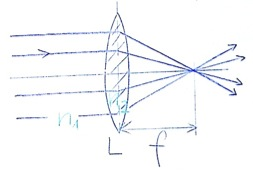
\includegraphics{Bild253} \\
	$n_1 , n_2$ Brechungsindizes \\
	$r_1 , r_2$ Kr�mmungsradien \\
	( $\oplus$ f�r M ; rechts von L )
	\begin{bsp*}[ note = Uhrglas ]
		\[ \begin{split}
			r_1 = r_2 \implies
				&\phi = 0 \\
				&f = 0
		\end{split} \]
		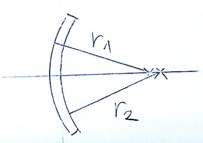
\includegraphics{Bild254}
	\end{bsp*}
	\begin{bsp*}
		\[
			f = \SI{10}{\centi\metre} = \SI{0.1}{\metre} \\
			\implies \phi = \SI{10}{\dioptre}
		\]
	\end{bsp*}
	
	\uline{Bildkonstruktion} \\
	$F_1$: Gegenstandsseitig \\
	$F_2$: Bildseitig \\
	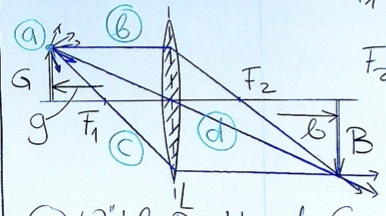
\includegraphics{Bild255} \\
	\begin{enumerate}[ label = ( \alph* ) ]
		\item W�hle Punkt auf $G$
		\item Parallellstrahl $\rightarrow F_2$
		\item Bremsstrahl $\rightarrow F_1$
		\item Kontrollstrahl (Zentrum)
	\end{enumerate}
	
	\uline{Abb. Gleichung}
	\[ \boxed{ \frac{1}{g} + \frac{1}{b} = \frac{1}{f} } \]
	
	\uline{Vorzeichen} \\
	Licht von links! \\
	$g > 0$ f�r $G$ links \\
	$b > 0$ f�r $B$ rechts \\
	Vergr�sserungsmassstab:
	\[ \boxed{ m = \frac{B}{G} = -\frac{b}{g} } \]
\end{rep*}

\section{Streulinsen ( \texorpdfstring{$f < 0$}{f < 0} )}
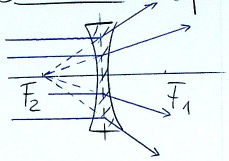
\includegraphics{Bild256} \\
virtueller Brennpunkt \\
neg. Dioprienzahl \\
Brillenglas mit $\phi < 0$ \\
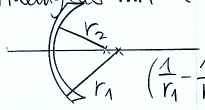
\includegraphics{Bild257}
\[ \left( \frac{1}{r_1} - \frac{1}{r_2} \right) < 0 \]

\subsection{Abbildung mit Streulinse}
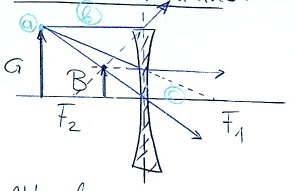
\includegraphics{Bild258} \\
\uline{Abb. Gl.}
\[
	f = \SI{3}{\deci\metre} \\
	g = \SI{4.4}{\deci\metre} \\
	\frac{1}{b} = \frac{1}{f} - \frac{1}{g} = \frac{-1}{3} - \frac{1}{4.4} = \dots \implies b = -1.7
\]

\section{Das menschliche Auge}
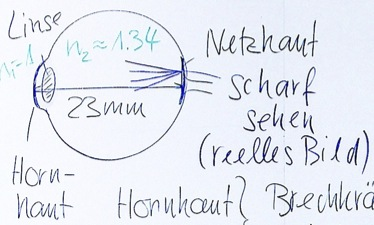
\includegraphics{Bild259} \\
\[
	\left. \begin{matrix*}[l]
		\text{Brechkr�fte} \\
		\text{Linse}
	\end{matrix*} \right\} \quad Brechkr�fte addieren
\]
zwei verschiedene Medien ($n_1 , n_2$) \\
$f_2 \neq f_1 \implies$ Brechkraft:
\[ \boxed{ \phi = \frac{n_2}{f_2} } \]

\subsection{Akkommodationsf�higkeit}
\subsubsection{Fernpunkt}
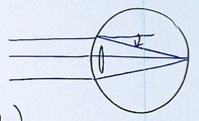
\includegraphics{Bild260}
\[
	f_2 = \SI{23}{\milli\metre} \\
	\left( \SI{60}{\dioptre} = \frac{1.34}{\SI{0.023}{\metre}} \right)
\]

\subsubsection{Nahpunkt}
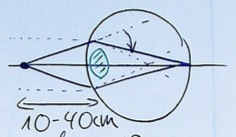
\includegraphics{Bild261}
$f_2 \approx \SI{18}{\milli\metre}$ \\
$\implies$ erh�hte Brechkraft ( $\sim \SI{74}{\dioptre}$ ) \\
\SI{25}{\centi\metre}: maximal scharfes Sehen

\subsection{Kurzsichtigkeit (myop)}
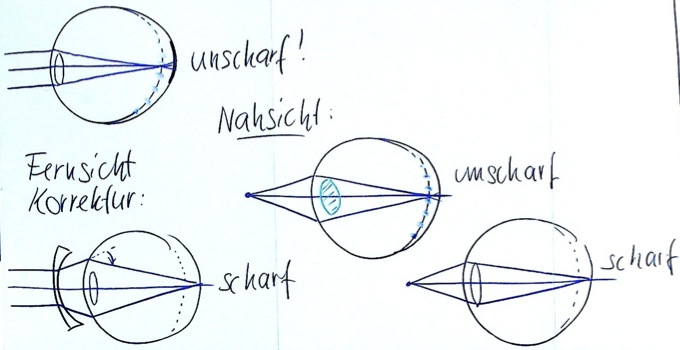
\includegraphics{Bild262}

\section{W�rmestrahlung}
\[ \lambda > \SI{750}{\nano\metre} \]
Thermodynamik: W�rmeaustausch via EM-Strahlung \\
Oberfl�che wichtig! \\
\enquote{schwarz}: keine Stralhung reflektiert \\
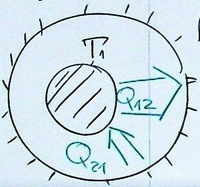
\includegraphics{Bild263} \\
schwarz $T_2 < T_1$ \\
$\overset{\rightsquigarrow}{\tau}$ TD-GGW ( $T_2 = T_1$ )

\subsection{Gesetz von Stefan-Boltzmann}
\begin{satz*}[ index = Gesetz von Stefan-Boltzmann , indexformat = {1!~23 3!12~} ]
	\[
		\boxed{ S = \sigma T^4 } \\
		\sigma = \SI{5.6E-8}{\watt\per\metre\squared\kelvin\tothe{4}}
	\]
\end{satz*}
\[
	\SI{300}{\kelvin} \rightarrow S = \SI{450}{\watt\per\metre\squared} \\
	\SI{500}{\kelvin} \rightarrow S = \SI{3.5}{\kilo\watt\per\metre\squared}
\]

\begin{rep*}[ note = W�rmestrahlung ]
	EM-Strahlung , $\lambda \gtrsim \SI{750}{\nano\meter}$ \\
	Erzeugung:
	\begin{itemize}
		\item Gitterschwingungen
		\item Molek�lvibrationen
	\end{itemize}
	Gesamte Abstrahlung eines \uline{schwarzen} K�rpers:
	\[ \boxed{ S = \sigma T^4 } \]
	(Gesetz von Stefan-Boltzmann)
	$\sigma = \SI{5.6E-8}{\watt\per\metre\squared\kelvin\tothe{4}}$
\end{rep*}

\subsection{Spektrum}
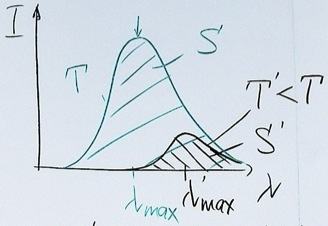
\includegraphics{Bild264} \\
Wien'sches Verschiebungsgesetz:
\[ \lambda_{\text{max}} \sim \frac{1}{T} \]
Kohlenbogenlampen:
\[
	T \approx \SI{2000}{\kelvin} \\
	\lambda_{\text{max}} \approx \SI{1450}{\nano\metre} (\text{IR})
\]
Sonne:
\[
	\lambda_{\text{max}} \approx \SI{510}{\nano\metre} \\
	\implies T \approx \SI{5900}{\kelvin}
\]

\section{R�ntgenstrahlung \texorpdfstring{$\lambda \approx \si{\angstrom}$}{}}
Erzeugung mit R�ntgenr�hre

\subsection{Spektrum einer \texorpdfstring{\ce{Mo}}{Mo}-Anode}
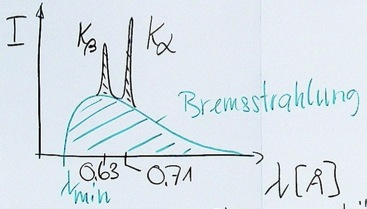
\includegraphics{Bild265} \\
Frequenz: $f = \frac{c}{\lambda}$ \\
$\lambda_{\text{min}}$: h�rteste Strahlung

\subsection{Messung}
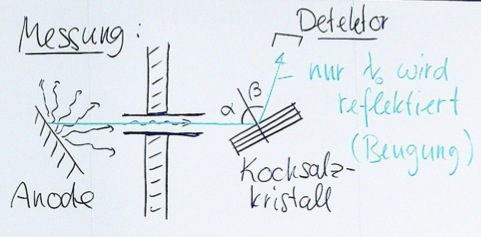
\includegraphics{Bild266}

\section{Atomphysik}
klassisches Atommodell \\
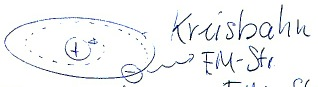
\includegraphics{Bild267} \\
Beschleunigung $\rightarrow$ EM-Strahlung \\
Energieverlust $\rightarrow$ instabil! \\
$\rightarrow$ Quantenphysik!!

\subsection{\texorpdfstring{\ce{Na}}{Na}-Atom}
( $Z = 11$ ) \\
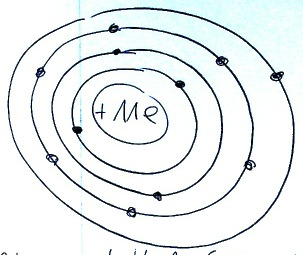
\includegraphics{Bild268} \\
Atom-Orbitale (Chemie) \\
Quantenzahlen \\
Hauptquantenzahl $n$
\[ n = 1 , 2 , 3 , \dots \]
Schale:
\[
	\begin{matrix*}[l]
		n = 1 : & K \\
		n = 2 : & L \\
		n = 3 : & M
	\end{matrix*}
\]
Drehimpulsquantenzahl $l$
\[
	\boxed{ l < n } \\
	l = \underbrace{0}_{s} , \underbrace{1}_{p} , \underbrace{2}_{d} , \dots
\]
physikalische Interpretation
\begin{itemize}[ label = $\rightarrow$ ]
	\item Wahrscheinlichkeit, wo sich \ce{e-} befindet
	\item phys. Messgr�ssen bestimmen
\end{itemize}
\begin{bsp*}[ note = Drehimpuls ]
	\[
		\vec{L} = \vec{r} \times \vec{p} \\
		\text{QM: } L = l \cdot \frac{h}{2\pi}
	\]
\end{bsp*}
Planck-konstante $h = \SI{6.62E-34}{\joule\second}$
\begin{bsp*}[ note = Energie ]
	$E( n , l )$ f�r jeden Zustand $n , l$
\end{bsp*}

\subsubsection{Besetzung dieser Atomorbitale}
\begin{itemize}
	\item Drehimpulsentartung: $2l + 1$ Pl�tze
	\item Spinentartung $\uparrow \downarrow \times 2$
\end{itemize}

\subsubsection{Pauli-Prinzip}
Nur 1 \ce{e-} pro Platz ( $2 \cdot ( 2l + 1 )$ ) \\
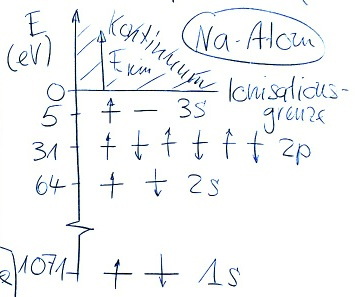
\includegraphics{Bild269} \\

\subsubsection{R�ntgenemission}
\begin{itemize}
	\item \uline{Bremsstrahlung} \\
		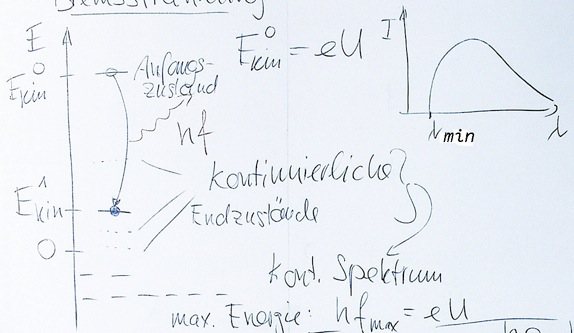
\includegraphics{Bild270} \\
		max. Energie: $hf_{\text{max}} = eU$
		\[ \boxed{ \lambda_{\text{min}} = \frac{c}{f_{\text{max}}} = \frac{hc}{eU} } \]
\end{itemize}

\subsubsection{Charakterischtische Strahlung}
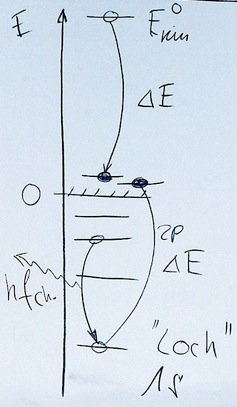
\includegraphics{Bild271} \\
$K_\alpha , K_\beta$? \\
Loch in $K$-Schale \\
Rekonstitution
\[
	\begin{matrix*}[l]
		2p \rightarrow 1s &K_\alpha \\
		3p \rightarrow 1s &K_\beta
	\end{matrix*}
\]
Loch in $L$-Schale
\[ 3p \rightarrow 2s \quad (\increment l = \pm 1 ) \]

\subsection{R�ntgenabsorbtion}
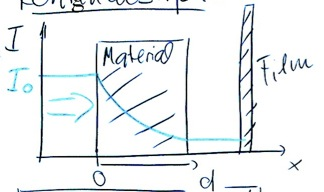
\includegraphics{Bild272}
\[ \boxed{ I(d) = I_0 e^{-\mu d} } \]
$\mu$: Absorbtionskoeffizient

\subsubsection{Prozess: Photoemission}
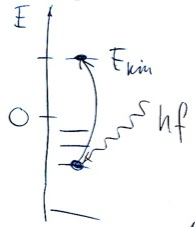
\includegraphics{Bild273}